\documentclass{article}

\usepackage{ctex, xeCJK, zxjatype}
\usepackage{metalogo, makecell, svg, amssymb, amsfonts, amsmath, physics, fancyhdr, geometry, graphicx, pdfpages, ragged2e, bm}
\usepackage{verbatim}
\newcommand{\R}{\mathbb{R}}
\newcommand{\rarr}{\rightarrow}
\newcommand{\lop}{Laplace算子}
\newcommand{\tRarr}{$\Rightarrow$}
\newcommand{\trarr}{$\Rightarrow$}
\newcommand{\filter}{\Gamma_{l,l'}}
\newcommand{\fn}[1]{\footnote{#1}}
\newcommand{\bs}[1]{\boldsymbol{#1}}
\newcommand{\iprod}[2]{\langle #1, #2 \rangle}
\newcommand{\define}{\textbf{Definition} }
\newcommand{\trm}{\textbf{Theorem} }
\newcommand{\alg}{\textbf{Algorithm} }
\newcommand{\cov}{\text{Cov}}
\newcommand{\bb}{\mathbb}
\newtheorem{theorem}{Theorem}[section]
\newtheorem{lemma}[theorem]{Lemma}
\newtheorem{proposition}[theorem]{Proposition}
\newtheorem{corollary}[theorem]{Corollary}
\newtheorem{definition}[theorem]{Definition}

\newenvironment{proof}[1][Proof]{\begin{trivlist}
\item[\hskip \labelsep {\bfseries #1}]}{\end{trivlist}}
% \newenvironment{definition}[1][Definition]{\begin{trivlist}
% \item[\hskip \labelsep {\bfseries #1}]}{\end{trivlist}}
\newenvironment{example}[1][Example]{\begin{trivlist}
\item[\hskip \labelsep {\bfseries #1}]}{\end{trivlist}}
\newenvironment{idea}[1][Idea]{\begin{trivlist}
\item[\hskip \labelsep {\bfseries #1}]}{\end{trivlist}}
\newenvironment{remark}[1][Remark]{\begin{trivlist}
\item[\hskip \labelsep {\bfseries #1}]}{\end{trivlist}}
\renewcommand{\cal}{\mathcal}
\usepackage[hidelinks, bookmarks]{hyperref} % add index hyper-links
\newcommand{\coro}{\textbf{Corollary} }
\newcommand{\tgt}{\textbf{Target} }
\newcommand{\bt}[1]{\textbf{#1}}
\newcommand{\lp}{Lagrange Polynomial}
\newcommand{\np}{Newton Polynomial}
\newcommand{\where}{\text{where }}
\newcommand{\centerimage}[2]{
    \centerline{\includegraphics[width=#1\paperwidth]{#2}
    }
}
\let\titleoriginal\title           % save original \title macro
\newcommand{\thetitle}{}
\renewcommand{\title}[1]{          % substitute for a new \title
    \titleoriginal{#1}%               % define the real title
    \renewcommand{\thetitle}{#1}        % define \thetitle
}

\newCJKfontfamily\gothic{IPAexGothic}
\newCJKfontfamily\mincho{IPAexMincho}

\title{\textbf{开题报告}}
\author{莫文韬}
\date{\today}
% set plain style
\pagestyle{fancy}
\lhead{} 
\chead{} 
\rhead{} 
% \lfoot{\it Notes on Geometric Learning} 
\lfoot{\hyperref[contents]{\thetitle}} 
% \lfoot{\thetitle} 
\cfoot{}
\rfoot{\thepage} 


% Length to control the \fancyheadoffset and the calculation of \headline
% simultaneously
\newlength\FHoffset
\setlength\FHoffset{1cm}

\addtolength\headwidth{2\FHoffset}

\fancyheadoffset{\FHoffset}

% these lengths will control the headrule trimming to the left and right 
\newlength\FHleft
\newlength\FHright

% here the trimmings are controlled by the user
\setlength\FHleft{1cm}
\setlength\FHright{0cm}

% The new definition of headrule that will take into acount the trimming(s)
\newbox\FHline
\setbox\FHline=\hbox{\hsize=\paperwidth%
  \hspace*{\FHleft}%
  \rule{\dimexpr\headwidth-\FHleft-\FHright\relax}{\headrulewidth}\hspace*{\FHright}%
}
\renewcommand\headrule{\vskip-.7\baselineskip\copy\FHline}

\renewcommand{\headrulewidth}{0.7pt} % hline width
\renewcommand{\footrulewidth}{0.7pt} 

% set margin
\geometry{a4paper,scale=0.75}
\newcommand{\note}{\textbf{Note} }
% \usepackage{background}
% \backgroundsetup{scale=1, angle=0, opacity = 0.2, contents = {
%     \includegraphics[width=\paperwidth, keepaspectratio]
%     {bg2.jpg}
%     }
% }

\usepackage{caption}

\newcommand{\cfig}[2]{
    \begin{figure}[htbp]
    \centering
    \includegraphics[width=#2\textwidth]{#1}
\end{figure}
}

\begin{document}
\maketitle
\section*{ }
\label{contents}
\tableofcontents

\section{开题依据}


\begin{figure}[htbp]
    \caption{一个典型的VQA任务特征融合模型的Pipeline(Duplicated from MFB)}
    \centering
    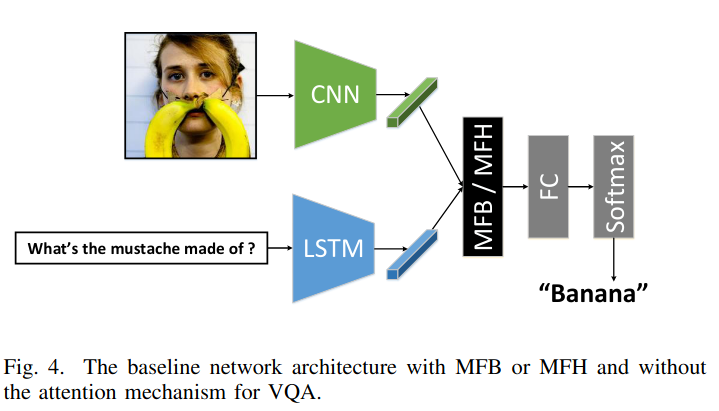
\includegraphics[width=\textwidth]{vqa-arch.png}
\end{figure}

Visual Question Answering(VQA)作为一个多模态任务这几年受到了广泛的关注, 一种经典的方法是是使用模态之间的特征融合方法来预测答案, 视觉和语言特征分别地进行特征提取后进行特征融合来得到全局特征. 最近的方法试图利用Co-Attention机制(MFH, MCAN, TRRNet etc.), 寻找并建模图像不同区域和问题不同词组之间的注意力和相关性, 来更好地得到多模态融合的特征(用于回答问题). 进一步地, Transformer作为顺序/特征种类无关的注意力机制被用于预训练的视觉-语言多模态特征学习的特征融合方法(ViLBERT, UNITER, OSCAR etc.), 可以将任意多的特征信息(除了视觉和文本特征, 还可以包括图像区域的语义标签的特征, 图像语义分割后的区域特征等等)作为Transformer输入序列的token进行特征融合. 此外, 作为一种特殊的注意力机制, 若给定场景/对象/词之间的关联信息, GNN也可以用于特征的融合. Co-Attention可以视作二分图上的图注意力机制, 而Transformers可以看做是完全图上的图注意机制.

\begin{figure}[htbp]
    \caption{利用Transformer进行特征融合(Duplicated from OSCAR)}
    \centering
    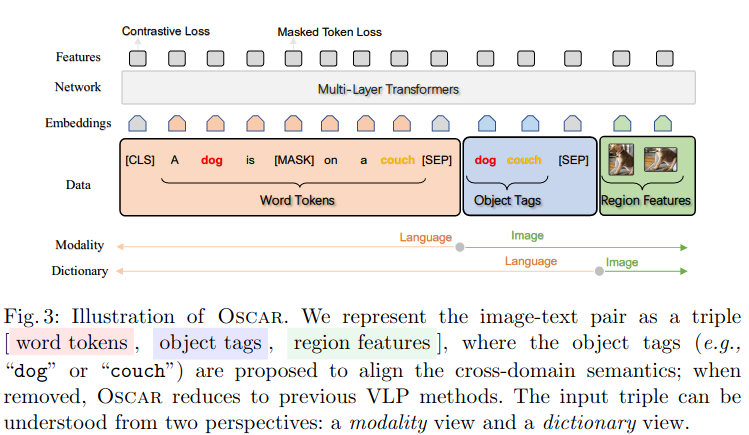
\includegraphics[width=\textwidth]{oscar-net.png}
\end{figure}


\begin{figure}[htbp]
    \centerline{
        \begin{tabular}{cc}
            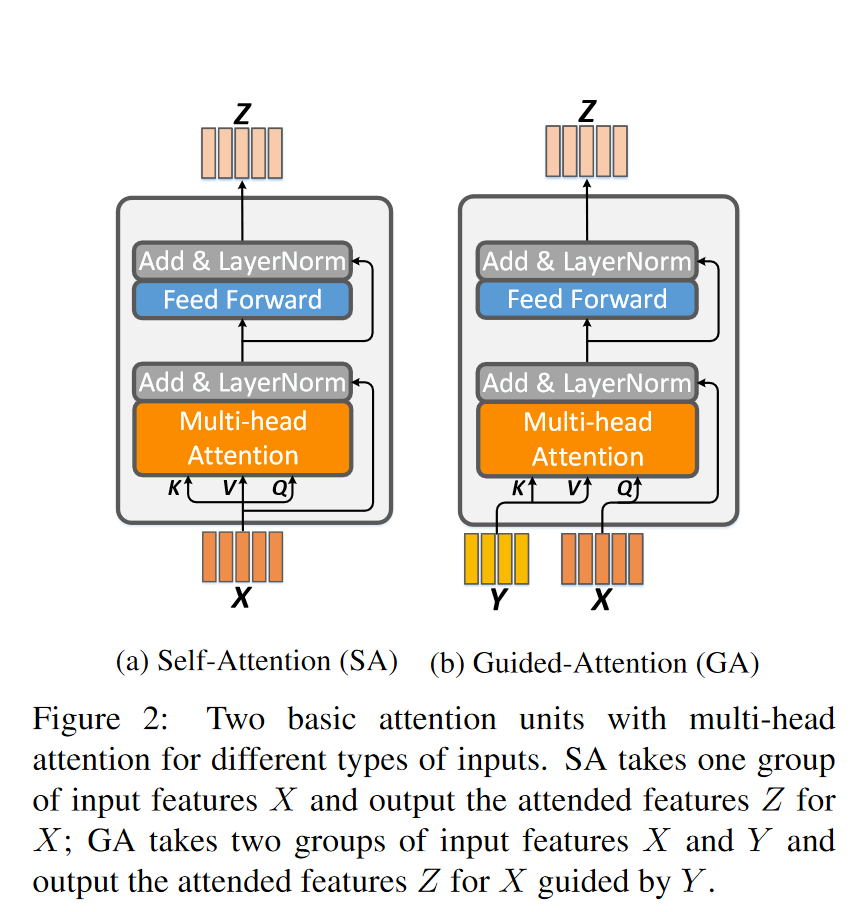
\includegraphics[width=0.55\textwidth]{mcan-mod.png}&
            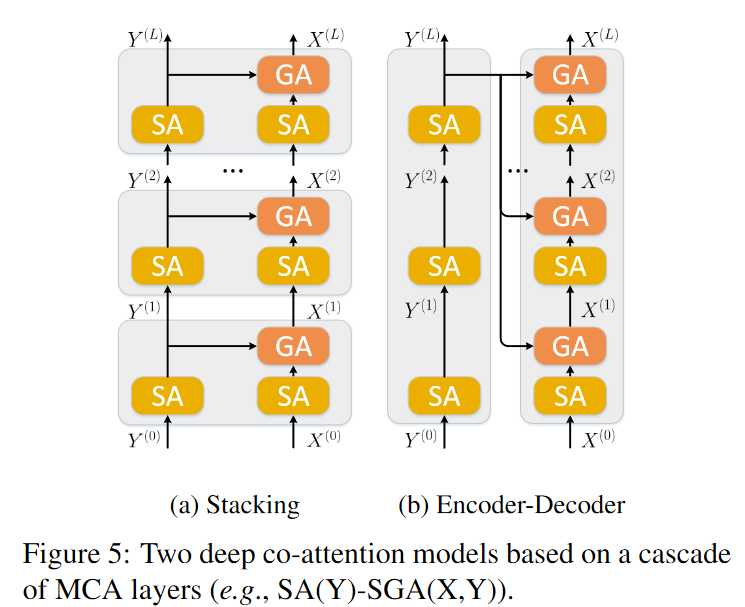
\includegraphics[width=0.55\textwidth]{mcan-arch2.png}
        \end{tabular}
    }
    \caption{利用Co-Attention进行特征融合(Dubplicated from MCAN)}
\end{figure}

另一方面, 为了减少Data Bias和不同数据集之间的Domain Gap, 也为了改进在预训练模型的性能, 一些新的视觉特征提取方法也被提出. 不同于广泛采用的Faster RCNN作为图片中对象和对象特征提取器的做法. Visual Commonsense RCNN提出利用整个数据集中对象之间的因果关系来改进提取到的特征, 减少因为Data Bias导致的表示模型学到的对象之间的伪因果关系. VinVL使用了超大数据集来与训练Faster RCNN, 来得到一个好的特征预提取器, 防止Domain Gap导致在和Target Domain不同视觉数据集/分布上的性能降低(无法检测某些未见到的物体中类等等). 问题是, 无法捕捉不同区域之间的不同关系, 只是考虑二分的Attention和稠密的完全Attention!

\begin{figure}[htbp]
    \caption{在Object Detector中加入因果的额外信息的一种框架(Duplicated from VC RCNN)}
    \centering
    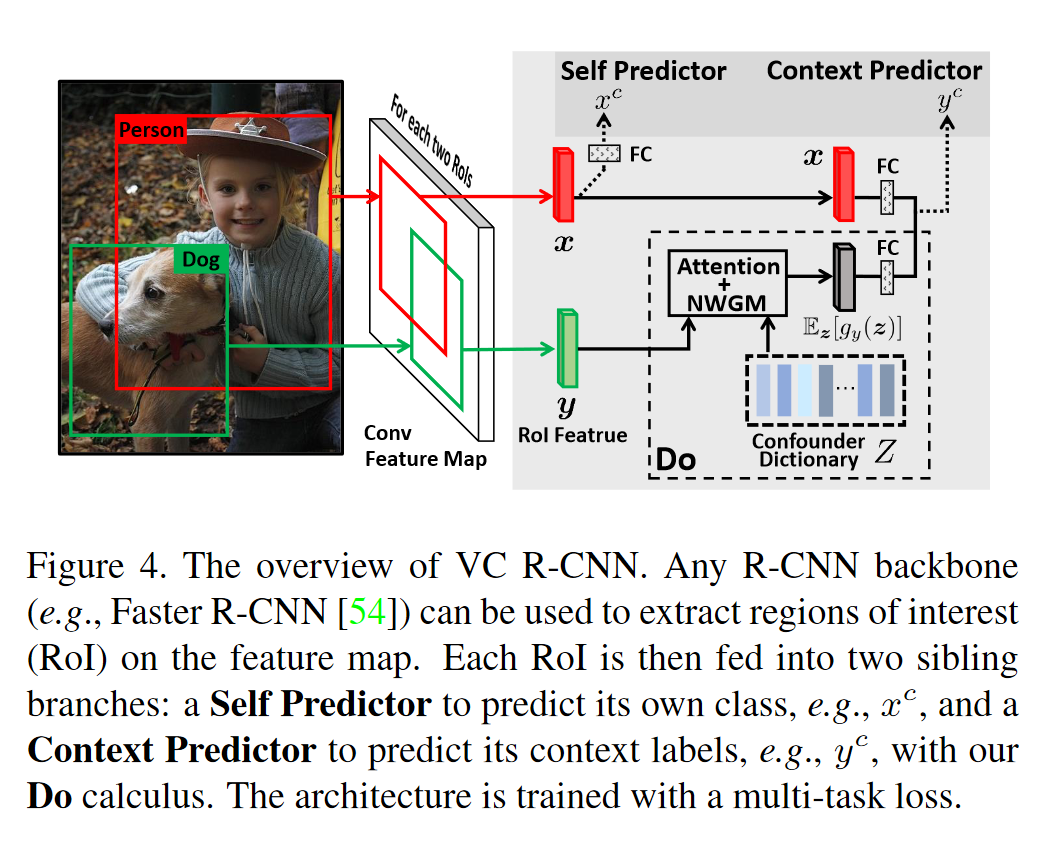
\includegraphics[width=0.7\textwidth]{vcrcnn-arch.PNG}
\end{figure}


\section{任务内容}

图神经网络是一种自然的融合不同图像-问题中不同的区域的特征的方法(这些区域可以是问题或对象标签的词嵌入, 也可以是图像的Grids/Regions/Semantic Regions特征等等), 它能考虑到不同区域之间的互动和关系(或者说某种注意力). 作为稀疏版的Transformers, GNN可以大大降低模型计算复杂度, 并且具有Transformers可以具有任意多输入区域, 同时对于输入区域的顺序具有Permutation Invariance. 作为一种带有额外信息的特征, 图的邻接矩阵如何获得是如何得到一个好的GNN融合的特征的关键. 自然的想法使用现成的方法检测场景中物体之间的互动/作用, 作为输入特征送入GNN进行融合. 端到端地学习邻接矩阵可能是另一种更优的解决方案. DGCNN的工作证明了, 在网络计算过程中使用动态图(邻接矩阵)是可行(可优化)且高效的. 这可能意味着优化一个好的特征映射可以得到好的邻接矩阵, 所以使用端到端的动态图训练可能是一个好的选择.

Sample reweighting? GPNN? minimize L1-norm? k-thresholding? kWTA?

\section{任务方案及可行性分析}

\textbf{Dynamic Graph Attention} 不同于传统GNN的输入邻接矩阵是固定的, 我们可以采用动态建立的图来作为邻接矩阵, 具体地, 对于每一层选取特征空间上的kNN作为邻接点
\begin{equation}
    a_{ij}=\bs{1}[d(i,j)\in topK(\{d(i, u)| u\in V\})]
\end{equation}
其中距离函数$d(i,j)=d(\bs h_i, \bs h_j)$,
以及每一层的Forward Pass
\begin{equation}
    x'_i = \frac 1 {|N(i)|} \sum_{j\in N(i)} f(s_i, s_j-s_i), s_i = \phi(x_i)
\end{equation}
或者使用Multi-head注意力机制(GAT)
\begin{equation}
    \vec{h}_{i}^{\prime}=\|_{k=1}^{K} \sigma\left(\sum_{j \in \mathcal{N}_{i}} \alpha_{i j}^{k} \mathbf{W}^{k} \vec{h}_{j}\right)
\end{equation}
其中注意力coefficient为
\begin{equation}
    \alpha_{i j}=\frac{\exp \left( \sigma \left(\overrightarrow{\mathbf{a}}^{T}\left[\mathbf{W} \vec{h}_{i} \| \mathbf{W} \vec{h}_{j}\right]\right)\right)}{\sum_{k \in \mathcal{N}_{i}} \exp \left( \sigma \left(\overrightarrow{\mathbf{a}}^{T}\left[\mathbf{W} \vec{h}_{i} \| \mathbf{W} \vec{h}_{k}\right]\right)\right)}
\end{equation}

\cfig{gat-arch.png}{1.0}

\textbf{Semantic Label as Fusion Input}

根据OSCAR模型的研究, 使用输入图像区域的标签作为VQA任务的特征融合提高了模型的性能和表达力, 并且可以自然地嵌入到上述的特征融合方法中作为一个图节点的输入. 我们可以选择使用预训练的词嵌入(Word2Vec, GLoVe等等)来得到一个节点特征并且和图像区域特征和问题特征三者一起进行融合.


\section{Reference}

\begin{enumerate}
    \item Li, Xiujun, et al. "Oscar: Object-semantics aligned pre-training for vision-language tasks." European Conference on Computer Vision. Springer, Cham, 2020.
    \item Chen, Yen-Chun, et al. "Uniter: Universal image-text representation learning." European Conference on Computer Vision. Springer, Cham, 2020.
    \item Yu, Zhou, et al. "Deep modular co-attention networks for visual question answering." Proceedings of the IEEE/CVF Conference on Computer Vision and Pattern Recognition. 2019.
    \item Pennington, Jeffrey, Richard Socher, and Christopher D. Manning. "Glove: Global vectors for word representation." Proceedings of the 2014 conference on empirical methods in natural language processing (EMNLP). 2014.
    \item Wang, Yue, et al. "Dynamic graph cnn for learning on point clouds." Acm Transactions On Graphics (tog) 38.5 (2019): 1-12.
    \item Veličković, Petar, et al. "Graph attention networks." arXiv preprint arXiv:1710.10903 (2017).
    \item Wang, Tan, et al. "Visual commonsense r-cnn." Proceedings of the IEEE/CVF Conference on Computer Vision and Pattern Recognition. 2020.
    \item Zhang, Pengchuan, et al. "VinVL: Making Visual Representations Matter in Vision-Language Models." arXiv preprint arXiv:2101.00529 (2021).
    \item Lu, Jiasen, et al. "Vilbert: Pretraining task-agnostic visiolinguistic representations for vision-and-language tasks." arXiv preprint arXiv:1908.02265 (2019).
    \item Yang, Xiaofeng, et al. "TRRNet: Tiered Relation Reasoning for Compositional Visual Question Answering."
    \item Yu, Zhou, et al. "Beyond bilinear: Generalized multimodal factorized high-order pooling for visual question answering." IEEE transactions on neural networks and learning systems 29.12 (2018): 5947-5959.

\end{enumerate}


\end{document}